\documentclass[../finalreport.tex]{subfiles}

\begin{document}

\par Étudions l'évolution de la richesse des agents dans le cas particulier où la variable connue par l'initié est $L = \ln \left( S_T^{1} \right) - \ln \left( S_T^{2} \right)$ : l'initié connait la proportion qu'auront les prix de deux actifs risqués au temps $T$. Il est possible de vérifier que dans ce cas, toutes les hypothèses techniques nécessaires à l'établissement de la solution du problème d'optimisation sont vérifiées.

\par Pour simplifier et rendre exploitable les calculs, nous nous plaçons en outre dans le cas où les paramètres $b, \sigma$, et $r$ du modèle sont constants.

\subsubsection{Calcul explicite des richesses}

\par Dans ce cas, nous pouvons expliciter la variable $L$ : les prix du marchés sont donnés par 
\begin{displaymath}
\begin{cases}
S_t^1 &= S_0^1 e^{ \left( b_1 - \frac{1}{2} ||\sigma_1||^2 \right) t + \left( \sigma_1, W \left( t \right) \right) }  \\
S_t^2 &= S_0^2 e^{ \left( b_2 - \frac{1}{2} ||\sigma_2||^2 \right) t + \left( \sigma_2, W \left( t \right) \right) }
\end{cases}
\end{displaymath}

\par Donc
\begin{displaymath}
L = \underbrace{\ln \left( \frac{S_0^1}{S_0^2} \right) + \left( \left( b_1 - b_2 \right) - \frac{1}{2} \left(||\sigma_1||^2 - ||\sigma_2|^2 \right) \right) T}_{=: \beta} + \left( \underbrace{\sigma_1 - \sigma_2}_{=: \gamma}, W \left( T \right) \right)
\end{displaymath}

\par Ainsi, $L$ est une variable gaussienne. La loi conditionnelle de $L$ sachant $\mathcal{F}_t$ s'exprime donc comme une loi gaussienne $\mathcal{N} \left( \beta + \left( \gamma, W \left( t \right) \right), ||\gamma||^2 \left( T - t \right) \right)$ qui est bien absolument continue comme annoncé dans la proposition~\ref{proposition_l}. Reprenons cette proposition dans ce cas particulier pour expliciter $l$. La densité conditionnelle de la loi de $L$ sachant $\mathcal{F}_t$ est donc celle d'une loi normale : 
\begin{displaymath}
p \left( t, x \right) = \frac{1}{ ||\gamma|| \sqrt{2 \pi} \sqrt{T - t}} \underbrace{e^{-\frac{1}{2} \frac{\left( x - \beta - \left( \gamma, W \left( t \right) \right) \right)^2}{||\gamma||^2 \left( T - t \right)}}}_{ =: f \left( t, W \left( t \right) \right)}
\end{displaymath}

\par Nous allons montrer que ce processus est bien une martingale. Pour cela, nous fixons $x$ et dérivons $p$ : par Itô, nous avons :

\begin{displaymath}
	\begin{split}
	dp \left( t, x \right) &= d \left( \frac{1}{ ||\gamma|| \sqrt{2 \pi} \sqrt{T - t}} \right) f \left( t, W \left( t \right) \right) + \frac{1}{ ||\gamma|| \sqrt{2 \pi} \sqrt{T - t}} d f \left( t, W \left( t \right) \right) \\
	&= \frac{1}{2  ||\gamma|| \sqrt{2 \pi} \left( T - t \right)^{\frac{3}{2}}} f \left( t, W \left( t \right) \right) + \frac{1}{ ||\gamma|| \sqrt{2 \pi} \sqrt{T - t}} d f \left( t, W \left( t \right) \right)
	\end{split}
\end{displaymath}

\par La formule d'Itô nous permet aussi de dériver $f$ : 

\begin{displaymath}
	\begin{split}
	df \left( t, W \left( t \right) \right) &= f_{x}^{'} \left( t, W \left( t \right) \right) d W \left( t \right) + \left[ f_{t}^{'} \left( t, W \left( t \right) \right) + \frac{1}{2} f_{xx}^{''} \left( t, W \left( t \right) \right) \right] dt \\
	&=  \left[ \frac{\left( x - \beta - \left( \gamma, W \left( t \right) \right)\right)}{||\gamma||^2 \left( T - t \right)} \right] f \left( t, W \left( t \right) \right) \left( \gamma, d W \left( t \right) \right) + \left[ \frac{-1}{2 \left( T - t \right)} \right]f \left( t, W \left( t \right) \right) dt
	\end{split}
\end{displaymath}

\par Ainsi, les termes temporels se simplifient et 

\begin{displaymath}
dp \left( t, x \right) = \frac{\left( x - \beta - \left( \gamma, W \left( t \right) \right) \right)}{||\gamma||^3 \sqrt{2 \pi} \left( T - t \right)^{\frac{3}{2}}} f \left( t, W \left( t \right) \right) \left( \gamma, d W \left( t \right) \right)
\end{displaymath}

\par Ainsi, $p$ est bien une martingale et on a, comme dans la proposition, la formule 

\begin{displaymath}
p \left( t, x \right) = p \left( t, x \right) + \int_0^t \left( \alpha \left(s, x \right), dW \left( s \right) \right)
\end{displaymath}

\par Où

\begin{displaymath}
\alpha \left( t, x \right) = \frac{\left( x - \beta - \left( \gamma, W \left( t \right) \right) \right)}{||\gamma||^3 \sqrt{2 \pi} \left( T - t \right)^{\frac{3}{2}}} f \left( t, W \left( t \right) \right) \gamma
\end{displaymath}

\par Ainsi, nous pouvons expliciter $l$ : 

\begin{displaymath}
	\begin{split}
	l_t &= \frac{\alpha \left(t, L \right)}{p \left(t, L \right)} \\
	&= \dfrac{ \left( \dfrac{\left( L - \beta - \left( \gamma, W \left( t \right) \right) \right)}{||\gamma||^3 \sqrt{2 \pi} \left( T - t \right)^{\frac{3}{2}}} \right) f \left( t, W \left( t \right) \right) \gamma}{ \left( \dfrac{1}{ ||\gamma|| \sqrt{2 \pi} \sqrt{T - t}} \right) f \left( t, W \left( t \right) \right)} \\
	&= \frac{\left( \gamma, W \left( T \right) - W \left( t \right) \right) \gamma}{||\gamma||^2 \left( T - t \right)} \quad \text{car } L - \beta = \left( \gamma, W \left( T \right) \right)
	\end{split}
\end{displaymath}

\par Or nous savons que le processus $Y$, inversement proportionnel à la richesse des agents, est, en vertu des formules présentées dans la section précédente :
\begin{displaymath}
Y \left( t \right) = 
\begin{cases}
e^{- \left( \eta, W_{t} \right)-\frac{1}{2} t {\| \eta \|}^{2}} =: Y_0 \left( t \right) & \text{pour le non initié} \\
e^{- \int_{0}^{t} \left( l_{s} + \eta, dW_{s} - l_s ds \right) - \frac{1}{2} \int_{0}^{t} {\| l_{s} + \eta \|}^{2} ds} & \text{pour l'initié}
\end{cases}
\end{displaymath}

\par Donc le coefficient de proportionnalité entre la richesse des deux agents est : 

\begin{displaymath}
	\begin{split}
	\frac{1}{Z \left( t \right)} &:= \frac{Y \left( t \right)}{Y_0 \left( t \right)} \\
	 &= \frac{e^{- \int_{0}^{t} \left( l_{s} + \eta, dW_{s} - l_s ds \right) - \frac{1}{2} \int_{0}^{t} {\| l_{s} + \eta \|}^{2} ds}}{e^{- \left( \eta, W_{t} \right)-\frac{1}{2} t {\| \eta \|}^{2}}} \\
	&= \frac{e^{- \int_{0}^{t} \left[ \left( l_s, dW_{s} \right) + \left( \eta, dW_{s} \right) - {\| l_{s} \|}^{2} ds - \left( \eta, l_s\right) ds \right]  - \frac{1}{2} \int_{0}^{t} \left[ {\| l_{s} \|}^{2} + {\| \eta \|}^{2} + 2 \left(l_s, \eta \right) \right] ds}}{e^{- \left( \eta, W_{t} \right)-\frac{1}{2} t {\| \eta \|}^{2}}} \\
	&= e^{- \int_{0}^{t} \left[ \left( l_s, dW_{s} \right) ds \right] + \frac{1}{2} \int_{0}^{t} {\| l_{s} \|}^{2} ds}
	\end{split}
\end{displaymath}

\par Ainsi, 

\begin{displaymath}
d \log \left( Z \left( t \right) \right) = \left(l_s, d W_s \right) - \frac{1}{2} {\| l_{s} \|}^{2} ds
\end{displaymath}

\par Mais remarquons qu'aussi par définition de $l$, 

\begin{displaymath}
d p \left( t, L \right) =  p \left( t, L \right) \left( l_s, d W_t \right)
\end{displaymath}

\par Donc par Itô :

\begin{displaymath}
d \log \left( p \left( t, L \right) \right) = \left(l_s, d W_s \right) - \frac{1}{2} {\| l_{s} \|}^{2} ds = d \log \left( Z \left( t \right) \right)
\end{displaymath}

\par De là, $\frac{Z \left( t \right)}{ p \left( t, L \right) }$ est constant, égal à sa valeur initiale :

\begin{displaymath}
	\begin{split}
	Z \left( t \right) &= \frac{Z \left( 0 \right)}{ p \left( 0, L \right) } p \left( t, L \right) \\
	&= \frac{\sqrt{T}}{\sqrt{T - t}} e^{\frac{- \left( \gamma, W \left( T \right) - W \left( t \right) \right)^2}{2 ||\gamma||^2 \left( T - t \right)} + \frac{\left( \gamma, W \left( T \right) \right)^2}{2 ||\gamma||^2 T }}
	\end{split}
\end{displaymath}

\par L'interprétation est intéressante : pour tout $t$, la valeur de proportionnalité entre la richesse de l'initié et celle du non-initié correspond - à une constante initiale près -  à la densité conditionnelle de la variable $L$ sachant $\mathcal{F}_t$, prise en $x = L$. Ce résultat est en réalité général, et correspond au point de vue présenté dans \cite{art5}.

\subsubsection{Analyse asymptotique de $Z$} \label{analyse_asympt}

\par Analysons le comportement de ce processus $Z$ afin d'étudier l'enrichissement de l'initié par rapport au non-initié. Remplaçons les termes browniens par leur espérance dans l'expression précédente de $Z$:

\begin{displaymath}
	\begin{split}
	Z \left( t \right) &\simeq \frac{\sqrt{T}}{\sqrt{T - t}} e^{\left( \frac{- \| \gamma \|^2 \left( T  - t \right) }{2 \| \gamma \|^2 \left( T - t \right)} + \frac{\| \gamma \|^2 T }{2 \| \gamma \|^2 T } \right) } \\
	&= \frac{\sqrt{T}}{\sqrt{T - t}}
	\end{split}
\end{displaymath}

\par Nous voyons qu'au temps final considéré,

\begin{displaymath}
	\begin{split}
	Z \left( A \right) &\simeq \frac{\sqrt{T}}{\sqrt{T - A}} \\
	&\xrightarrow[A \to T]{} + \infty
	\end{split}
\end{displaymath}

\par Nous retrouvons ainsi le phénomène d'explosion en temps fini mentionné précédemment : plus $A$ se rapproche de $T$, plus la richesse finale de l'initié est grande par rapport à celle du non-initié.

\subsubsection{Test statistique}
\par Dans ce cas particulier, nous pouvons en outre construire un test statistique afin de détecter si l'agent est ou non un initié. Nous considérons les hypothèses suivantes : \emph{l'agent n'est pas initié} (i.e. l'information $L$ possédée dès le début de son investissement appartient en réalité à l'ensemble d'informations dont disposent tous les autres investisseurs sur le marché), contre l'hypothèse alternative : \emph{l'agent est un initié}, (i.e. l'agent est le seul à disposer de cette information). \\

Le test est donc décrit de manière suivante : 
\begin{itemize}
\item $H_0 : L \in \mathcal{F}_0$ (l'agent est un non initié) \
\item $H_1 : L \notin \mathcal{F}_0$ (l'agent est un initié)
\end{itemize}
\

Pour décider quelle hypothèse choisir, nous comparons les consommations optimales des agents, données par la formule $\displaystyle R_t c^*_t = \frac{X_0}{A+1}\frac{1}{Y}(t)$.\\
\mathleft
\begin{equation*}
\begin{cases} \log R_t c^*_t = \log(\frac{X_0}{A+1}) + \frac{1}{2}  \int_{0}^{t} ||\eta_s||^2 ds + \int_{0}^{t} \eta_s dW_s , \text{ sous } H_0\\

\log R_t c^*_t = \log(\frac{X_0}{A+1}) + \frac{1}{2}  \int_{0}^{t} ||\eta_s||^2 ds + \int_{0}^{t} \eta_s dW_s + \log q(t, L), \text{ sous } H_1 \end{cases}
\end{equation*}

Nous partitionnons $[0, T]$ en $0 \leq t_0 < t_1 < \dots <t_n = T$ et définissons 
\mathcenter
\begin{equation*}
Y_i := \log(R_{t_{i+1}} c_{t_{i+1}}) - \log (R_{t_{i}}c_{t_{i}}), \quad 0 \leq i \leq n-1.
\end{equation*}

En supposant que les paramètres $b, r$ et $\sigma$ sont déterministes, nous avons sous $H_0$,
\begin{equation*}
\displaystyle Y_i =  \frac{1}{2} \int_{t_i}^{t_{i+1}} ||\eta_s||^2 ds + \int_{t_i}^{t_{i+1}} \eta_s dW_s 
\end{equation*}
dont nous constatons qu'elle est une variable aléatoire gaussienne $\mathcal{N}\big(\frac{1}{2} \int_{t_i}^{t_{i+1}} ||\eta_s||^2 ds , \int_{t_i}^{t_{i+1}} ||\eta_s||^2 ds \big)$, tandis que sous $H_1$, nous avons le terme supplémentaire $\displaystyle \log\big(\frac{q(t_{i+1}, L)}{q(t_i, L)}\big)$.\\

Nous pouvons donc construire un test de région critique au niveau $\alpha = 0.05$ :
\begin{equation*}
RC_i = \Big\{ \omega : \big|Y_i (\omega) - \frac{1}{2} \int_{t_i}^{t_{i+1}} ||\eta_s||^2 ds \big| > 1.96 \sqrt{\int_{t_i}^{t_{i+1}} }\eta_s ds \Big\}
\end{equation*}

\par Remarquons que ce test dépend en réalité de la variable $L$ supposée connue par l'agent initié : il ne peut pas être utilisé en pratique.

\subsubsection{Simulations numériques}

\par Afin d'étudier numériquement les comportements des agents, nous avons implémenté ces formules en \emph{Python}. Par souci de généralité, nous avons choisi d'écrire notre code de la manière la plus générale et modulaire possible, c'est pourquoi nous décidons de ne pas le copier en annexe. Toutefois, il est disponible sur le \emph{repository Github} du projet (\url{https://github.com/lucas-broux/Projet-3A}).

\par Notre approche est la suivante : 
\begin{enumerate}
\item Calcul des prix (la formule est explicite).
\item Calcul de la richesse du non initié (ou plutôt du processus $\frac{1}{Y_0}$ ): selon la formule $ Y_0 \left( t \right) := e^{- \left( \eta, W_{t} \right)-\frac{1}{2} t {\| \eta \|}^{2}} $.
\item Calcul du processus $Z$ via la formule précédente $Z \left( t \right) = \frac{\sqrt{T}}{\sqrt{T - t}} e^{\frac{- \left( \gamma, W \left( T \right) - W \left( t \right) \right)^2}{2 ||\gamma||^2 \left( T - t \right)} + \frac{\left( \gamma, W \left( T \right) \right)^2}{2 ||\gamma||^2 T }}$
\item Calcul de la richesse de l'initié (ou plutôt du processus $\frac{1}{Y}$ ) par la formule $\frac{1}{Y} = \frac{Z}{Y_0}$ 
\end{enumerate}

\par Dans notre simulation (\emph{simulations\_diffusive\_model.py}), 
\begin{displaymath}
\begin{cases}
T &= 1 \\
A &= 0.95 \\
d &= 2 \\
r &= 0.1 \\
b &= \begin{bmatrix}
		0.1 & -0.05
	\end{bmatrix} \\
\sigma &= \begin{bmatrix}
			0.75 & 0 \\
			0 & 1
		  \end{bmatrix}
\end{cases}
\end{displaymath}

\par Les prix évoluent de la manière suivante :
\begin{figure}[H]
  \centering
    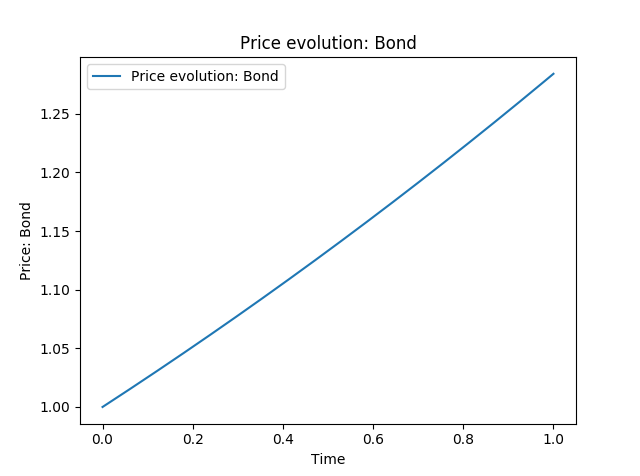
\includegraphics[width=0.7\textwidth]{images/simulation_1/price_0.png}
  \caption{prix de l'actif sans risque}
\end{figure}

\begin{figure}[H]
  \centering
    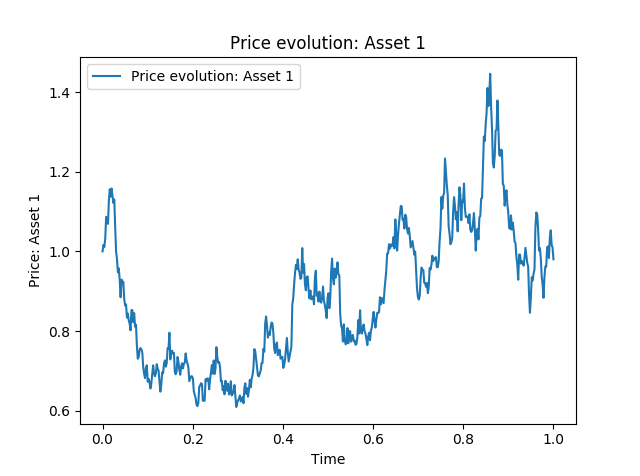
\includegraphics[width=0.7\textwidth]{images/simulation_1/price_1.png}
  \caption{prix de l'actif risqué 1}
\end{figure}

\begin{figure}[H]
  \centering
    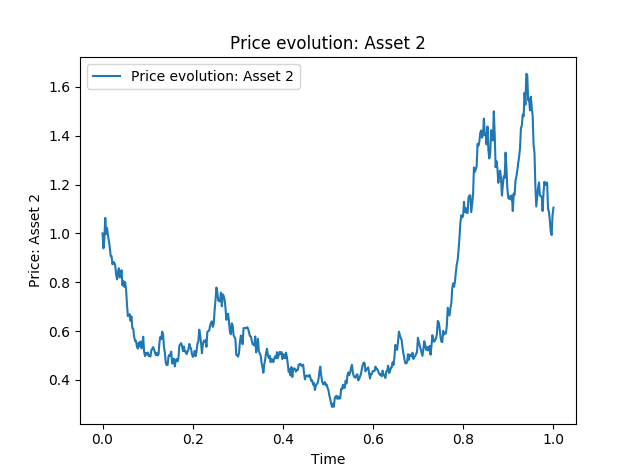
\includegraphics[width=0.7\textwidth]{images/simulation_1/price_2.png}
  \caption{prix de l'actif risqué 2}
\end{figure}

\par La valeur de la variable connue par l'initié est $L = -0.12$. Le processus $Z$ est ensuite calculé et comparé avec l'estimation produite dans la sous-partie \ref{analyse_asympt} :

\begin{figure}[H]
  \centering
    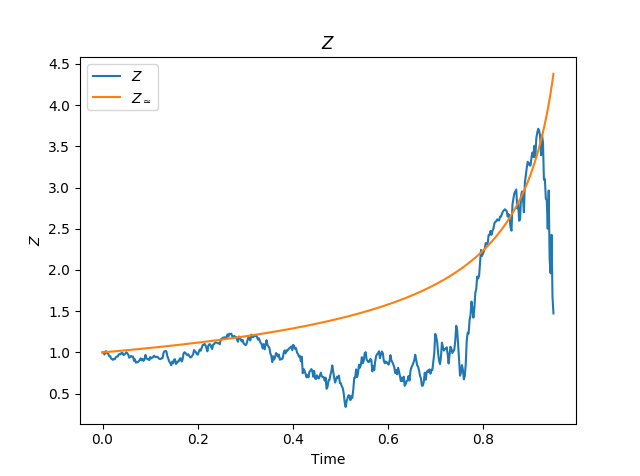
\includegraphics[width=0.7\textwidth]{images/simulation_1/compared_Z.png}
  \caption{$Z$ sur $\left[0; A \right]$}
\end{figure}

\par Nous constatons que, comme estimé, le processus $Z$ tend bien à diverger lorsque $t$ se rapproche de $T$. Nous pouvons enfin représenter l'évolution comparé de la richesse des deux agents :

\begin{figure}[H]
  \centering
    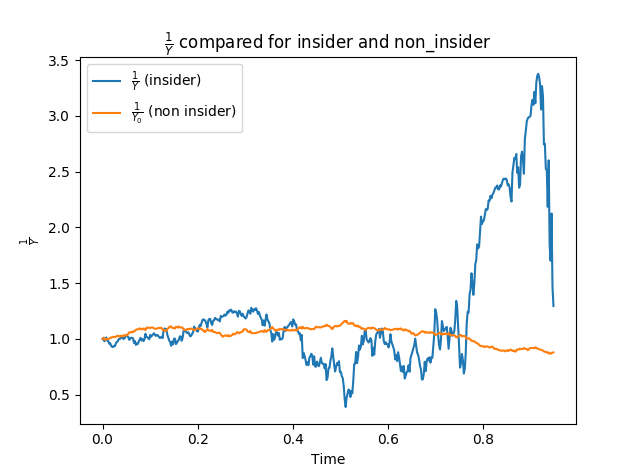
\includegraphics[width=0.7\textwidth]{images/simulation_1/compared_wealths.png}
  \caption{$\frac{1}{Y_0}$ et $\frac{1}{Y}$ sur $\left[0; A \right]$}
\end{figure}

\par Ainsi, l'initié tend à s'enrichir lorsque $t$ tend vers $A$ pour $A$ proche de $T$ : la connaissance de l'information $L$ permet à l'initié d'établir une meilleure stratégie que le non-initié.

\end{document}
